% !TEX root = thesis.tex

%%
%%
%% Discussion chapter
%%
%%

The contribution of this thesis is an empirical statistical analysis of the accuracy of the \gls{dkd}
as a tool for estimating the incidence risk of chronic diseases.
We examined the effect of several factors on the \gls{dkd} accuracy,
and we used several methods to measure the accuracy of the \gls{dkd} estimate,
as described in \Cref{sec:method:accuracy}.
We ran several scenarios to examine how variations in these factors which affect the incidence risk function,
the population distribution, and the sample size affect the accuracy of \gls{dkd} for estimation.
We compared two bandwidth selection techniques, \gls{silverman}'s rule of thumb,
and least-squares \glsentrylong{cv}.
We also compared these two techniques to an \gls{oracle},
which is an approximation of the theoretical optimal bandwidth.

As we discussed in \Cref{subsec:method:mise},
the \glsentrylong{mise} is the measure used by both \gls{silverman} and \gls{cv} for choosing the bandwidth.
In order to compare the results of different experiments which have different scales of \gls{risk} functions,
we normalized the \gls{mise} as \gls{nmise}. 
\Cref{fig:discussion:overall_nmise_boxplot} shows the overall distribution between experiments of the \gls{nmise}.
The \gls{nmise} for the \gls{oracle} selected bandwidth was, on average,
lower than for the other bandwidth selectors.
The \gls{cv} and \gls{silverman} selectors had similar performance.
All of these bandwidth selection techniques are optimized to minimize \gls{mise},
and so these results are what we expected.

The scale of the \gls{nmise} is much higher when the population is not uniform.
In particular, this seems to happen in two scenarios.
The first scenario occurs when the \gls{risk} function peak is far from the population peak, resulting in very few people in the high-risk area.
In a study with a real \gls{incident} \gls{risk},
this would have the effect of attenuating the actual \gls{risk}.
The second scenario where the \gls{nmise} is high occurs when the population density \gls{spread} takes its lowest values of 0.7 and 1.0.
This results in a highly variable denominator in the \gls{dkd} quotient,
leading to less stable results.
Although on average, the \gls{cv} and \gls{silverman} selectors have similar performance for the peaked populations,
the variance of the \gls{cv} selector is much higher.

\begin{figure}[htbp]
    \centering
    \begin{subfigure}[t]{0.45\textwidth}
        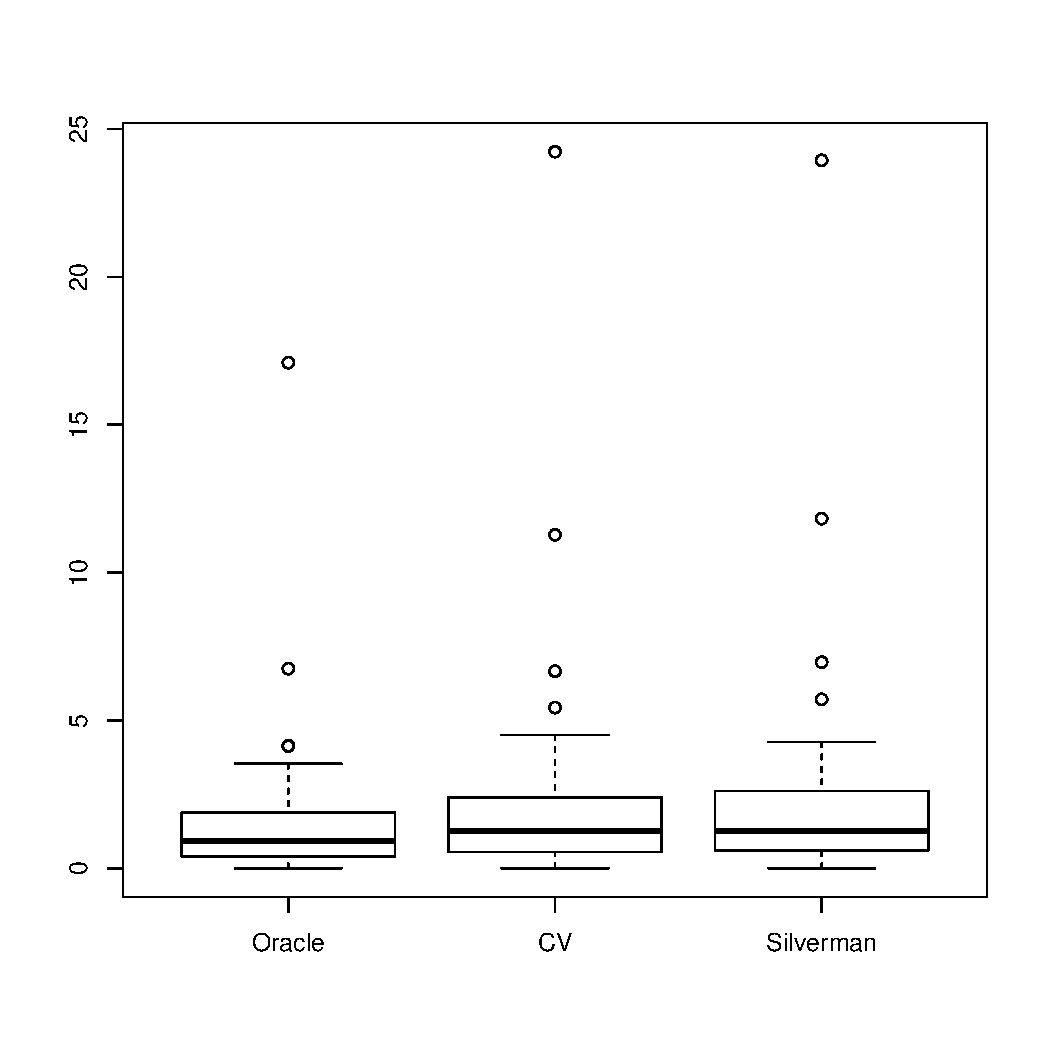
\includegraphics[width=\textwidth]{results/by_overall/normalized-mise-boxplot}
        \subcaption{Uniform populations}
        \label{fig:discussion:overall_nmise_boxplot:unif}
    \end{subfigure}
    \begin{subfigure}[t]{0.45\textwidth}
        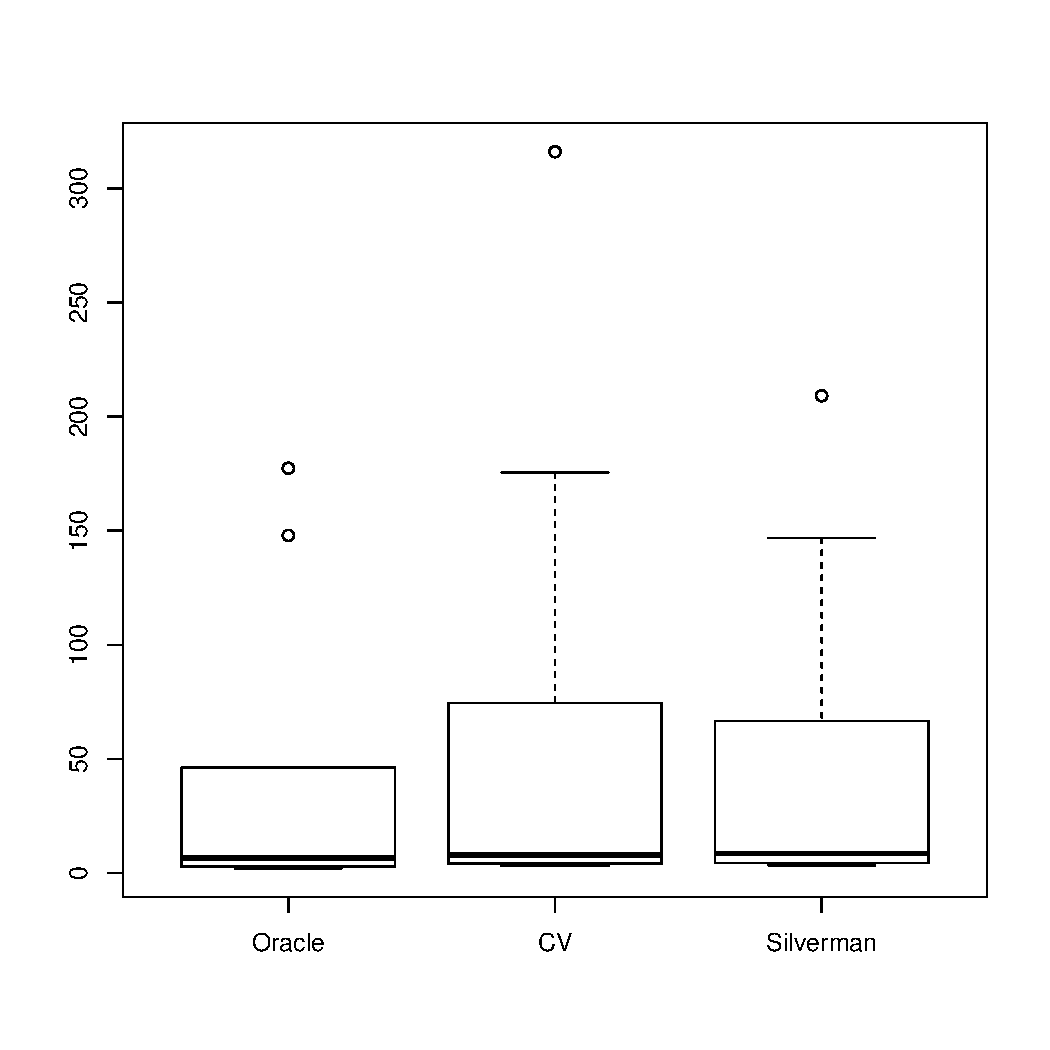
\includegraphics[width=\textwidth]{results/by_overall/normalized-mise-peakpop-boxplot}
        \subcaption{Peaked populations}
        \label{fig:discussion:overall_nmise_boxplot:peak}
    \end{subfigure}
    \caption{Overall distribution of \glsentryname{nmise}}
    \label{fig:discussion:overall_nmise_boxplot}
\end{figure}

\begin{figure}[htbp]
    \centering
    \begin{subfigure}[t]{0.45\textwidth}
        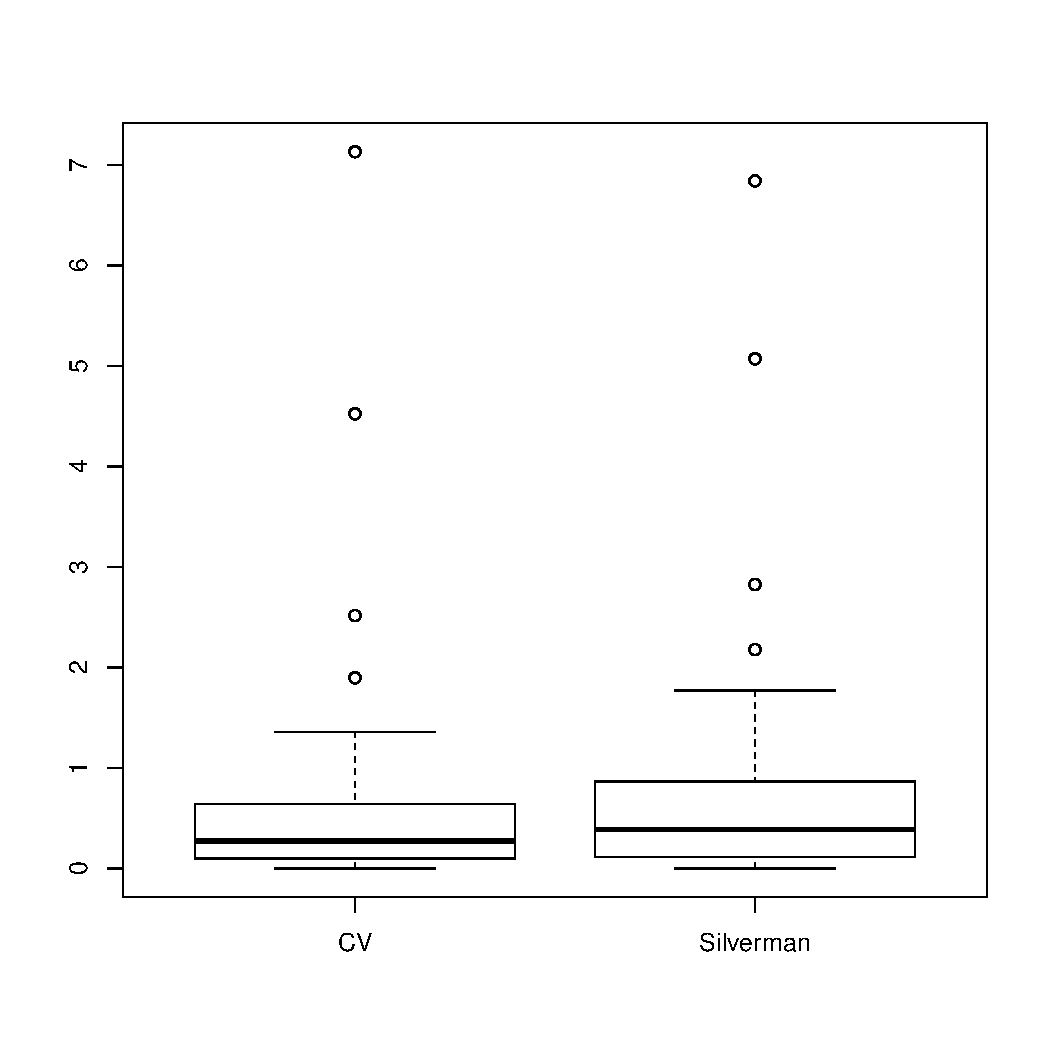
\includegraphics[width=\textwidth]{results/by_overall/normalized-mise-diff-boxplot}
        \subcaption{Uniform populations}
        \label{fig:discussion:overall_nmise_diff_boxplot:unif}
    \end{subfigure}
    \begin{subfigure}[t]{0.45\textwidth}
        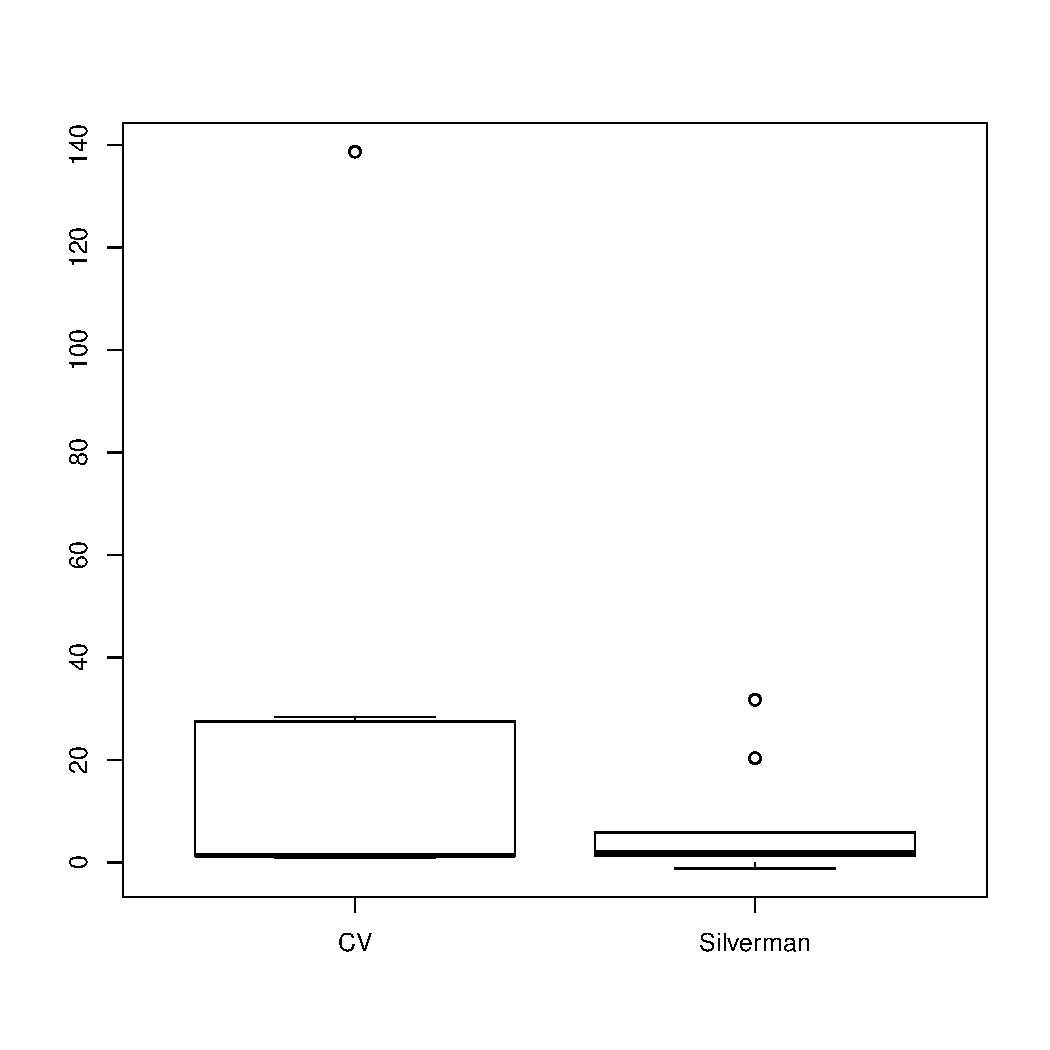
\includegraphics[width=\textwidth]{results/by_overall/normalized-mise-diff-peakpop-boxplot}
        \subcaption{Peaked populations}
        \label{fig:discussion:overall_nmise_diff_boxplot:peak}
    \end{subfigure}
    \caption{Overall distribution of \glsentryname{nmise} difference from the \Glsentryname{oracle}}
    \label{fig:discussion:overall_nmise_diff_boxplot}
\end{figure}

We now look at the \gls{miae}.
As mentioned in \Cref{subsec:method:miae},
the \glsentrylong{miae} is the natural measure that shows the average overall accuracy of the \gls{dkd} estimate of the \gls{risk} function.
By normalizing the \gls{miae}, we obtain the \gls{nmiae}.
Our theoretical optimal bandwidth \gls{h_opt} and our \gls{oracle} which is our estimation of it,
are based on minimizing \gls{mise}.
Also, both of \gls{silverman} and \gls{cv} are bandwidth selectors that attempt to minimize \gls{mise}.
It is not necessarily the case that a bandwith that minimizes \gls{ise} may also be the minimizer of \gls{iae}.
Nevertheless, our results show that for the types of \gls{risk} intensities we studied,
the \gls{cv} and \gls{silverman} selectors performed similarly to each other for \gls{nmiae}.
\Cref{fig:discussion:overall_nmiae_boxplot} shows the distribution of \gls{nmiae} over the entire set of experiments.
We note the large difference in scale between the experiments with uniform populations shown in \subref{fig:discussion:overall_nmiae_boxplot:unif} and those with peaked populations in \subref{fig:discussion:overall_nmiae_boxplot:peak}.


\begin{figure}[htbp]
    \centering
    \begin{subfigure}[t]{0.45\textwidth}
        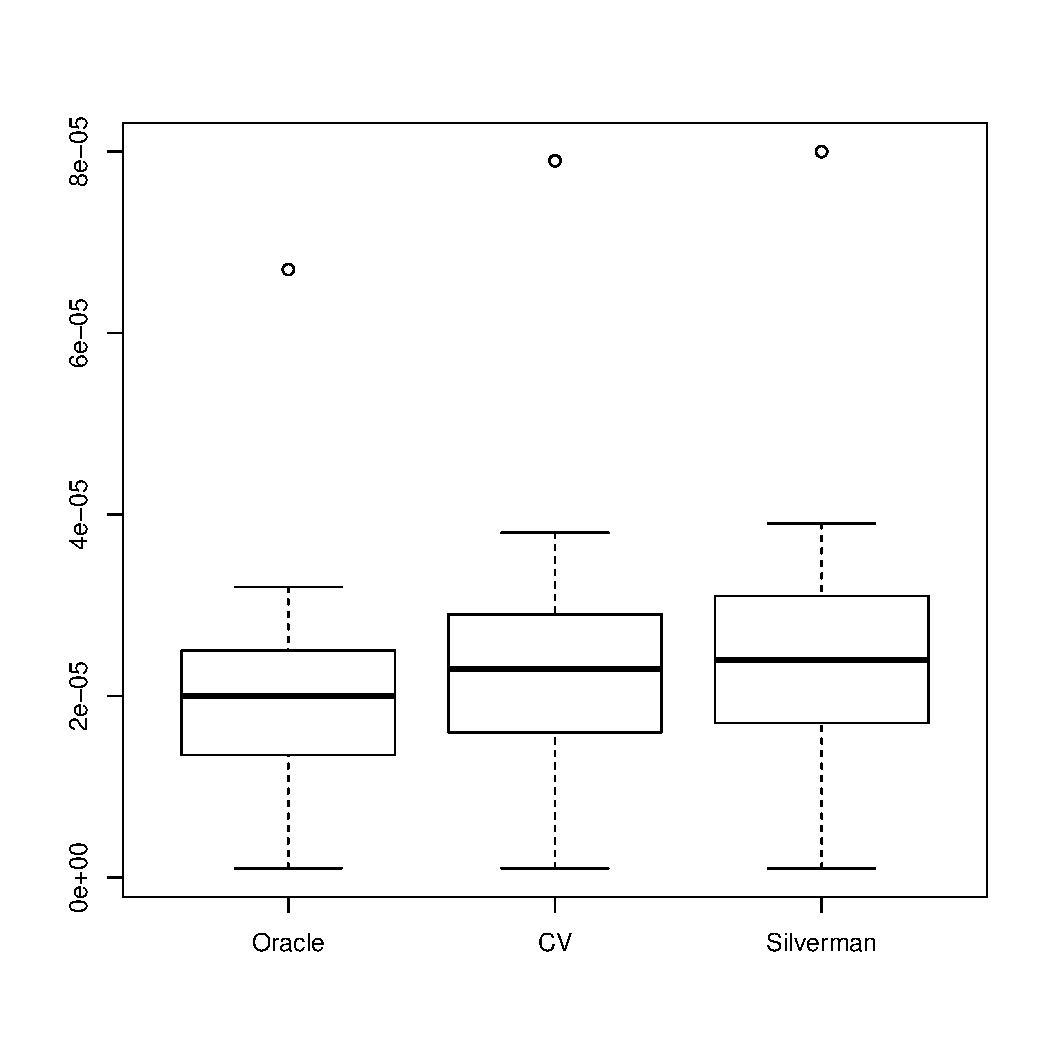
\includegraphics[width=\textwidth]{results/by_overall/normalized-miae-boxplot}
        \subcaption{Uniform populations}
        \label{fig:discussion:overall_nmiae_boxplot:unif}
    \end{subfigure}
    \begin{subfigure}[t]{0.45\textwidth}
        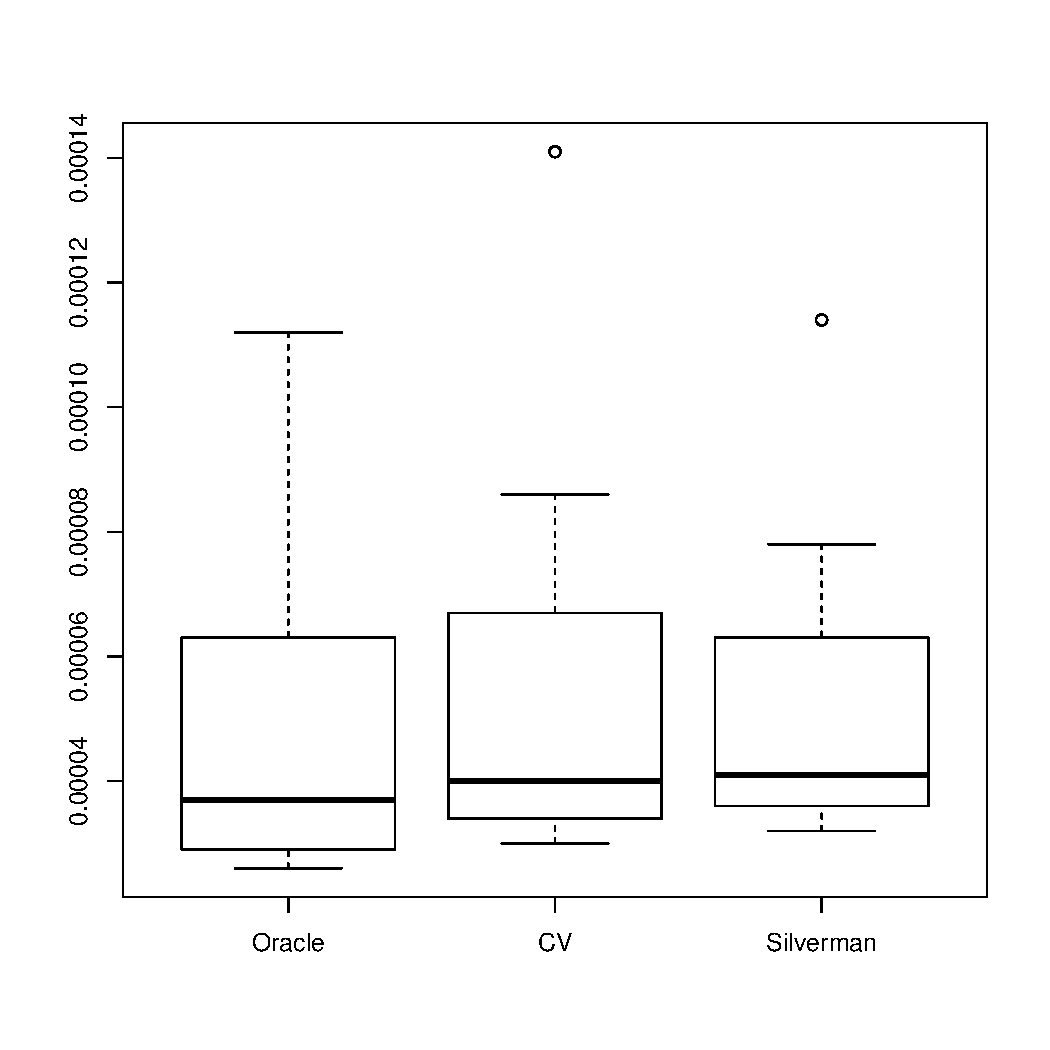
\includegraphics[width=\textwidth]{results/by_overall/normalized-miae-peakpop-boxplot}
        \subcaption{Peaked populations}
        \label{fig:discussion:overall_nmiae_boxplot:peak}
    \end{subfigure}
    \caption{Overall distribution of \glsentryname{nmiae}}
    \label{fig:discussion:overall_nmiae_boxplot}
\end{figure}

\begin{figure}[htbp]
    \centering
    \begin{subfigure}[t]{0.45\textwidth}
        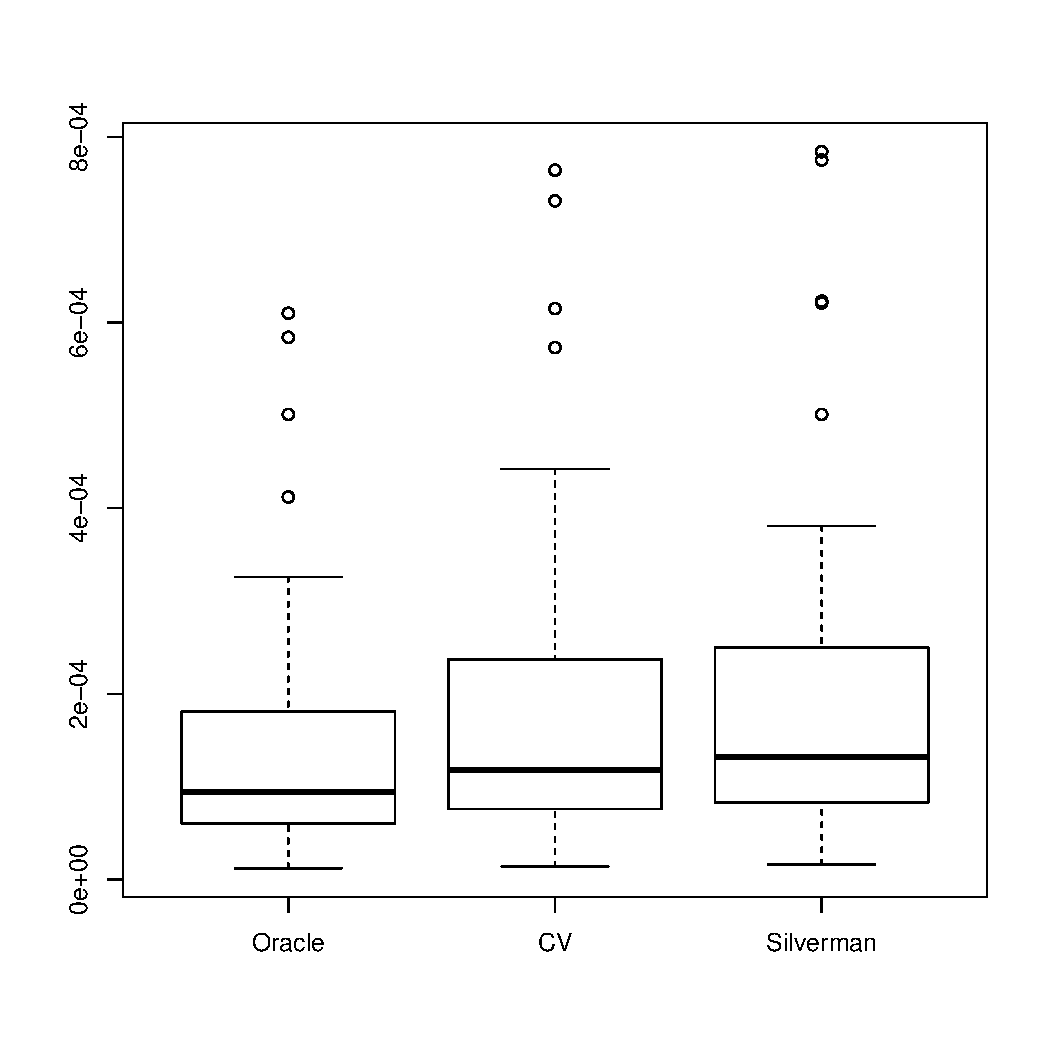
\includegraphics[width=\textwidth]{results/by_overall/normalized-sup-error-boxplot}
        \subcaption{Uniform populations}
        \label{fig:discussion:overall_nsup_boxplot:unif}
    \end{subfigure}
    \begin{subfigure}[t]{0.45\textwidth}
        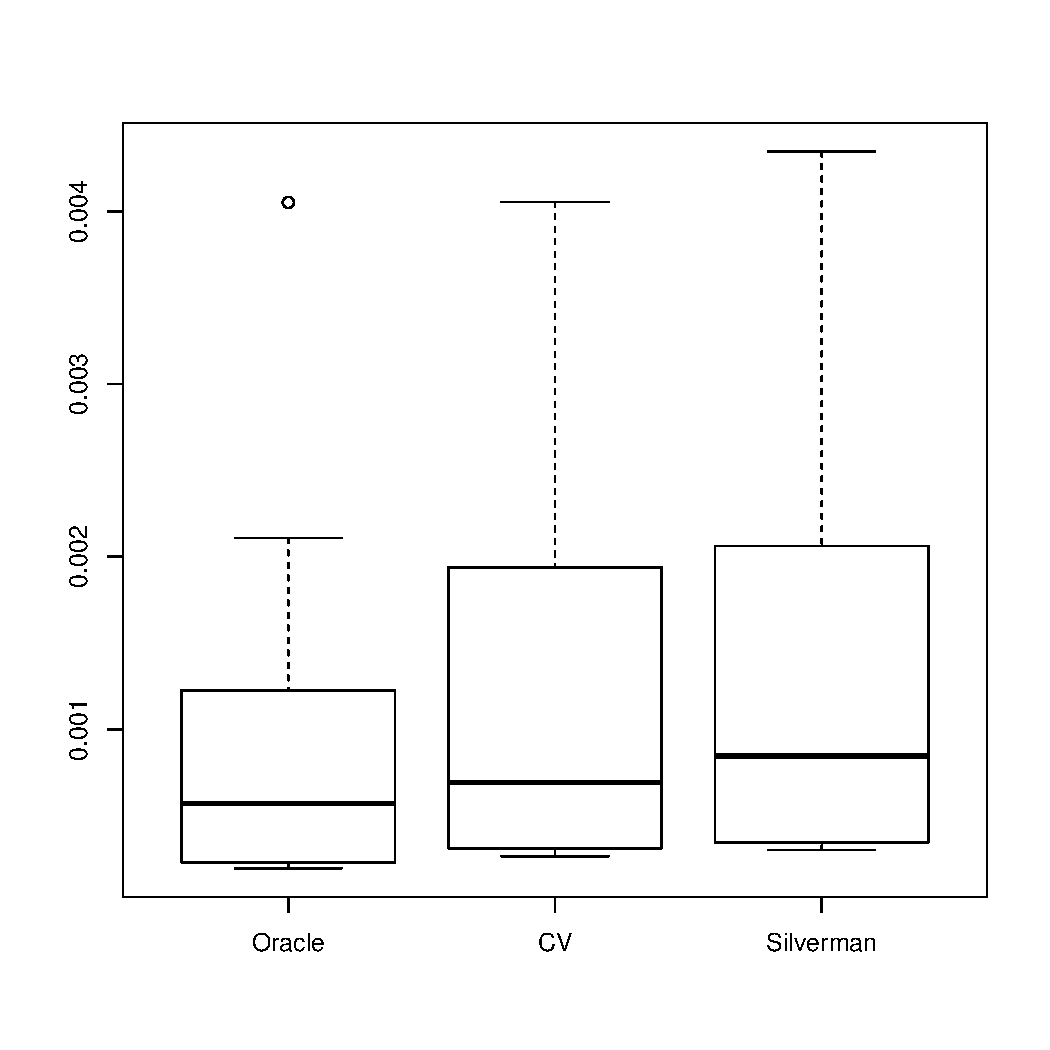
\includegraphics[width=\textwidth]{results/by_overall/normalized-sup-error-peakpop-boxplot}
        \subcaption{Peaked populations}
        \label{fig:discussion:overall_nsup_boxplot:peak}
    \end{subfigure}
    \caption{Overall distribution of \glsentryname{normalized supremum error}}
    \label{fig:discussion:overall_nsup_boxplot}
\end{figure}

Our \gls{supremum error} measure intuitively describes the expected worst case error of the \gls{dkd} estimate.
\Cref{fig:discussion:overall_nsup_boxplot} shows the overall distribution of the \gls{supremum error} over our experiments.
The results for uniform and peaked populations are shown in \Cref{fig:discussion:overall_nsup_boxplot:unif,fig:discussion:overall_nsup_boxplot:peak} respectively.
Why is the scale so much higher? See \Cref{sec:results:spread}.

\begin{figure}[htbp]
    \centering
    \begin{subfigure}[t]{0.45\textwidth}
        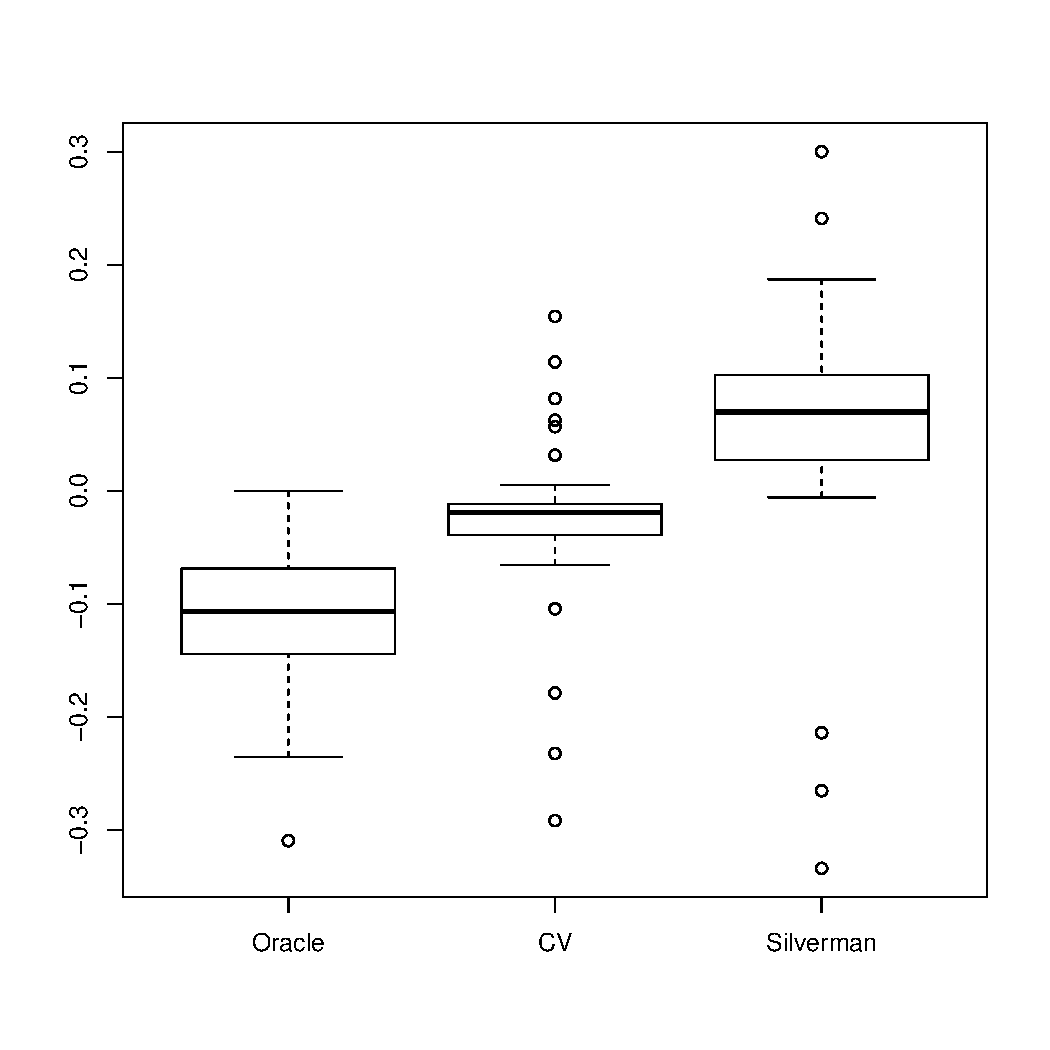
\includegraphics[width=\textwidth]{results/by_overall/relative-peak-bias-boxplot}
        \subcaption{Uniform populations}
        \label{fig:discussion:overall_peakbias_boxplot:unif}
    \end{subfigure}
    \begin{subfigure}[t]{0.45\textwidth}
        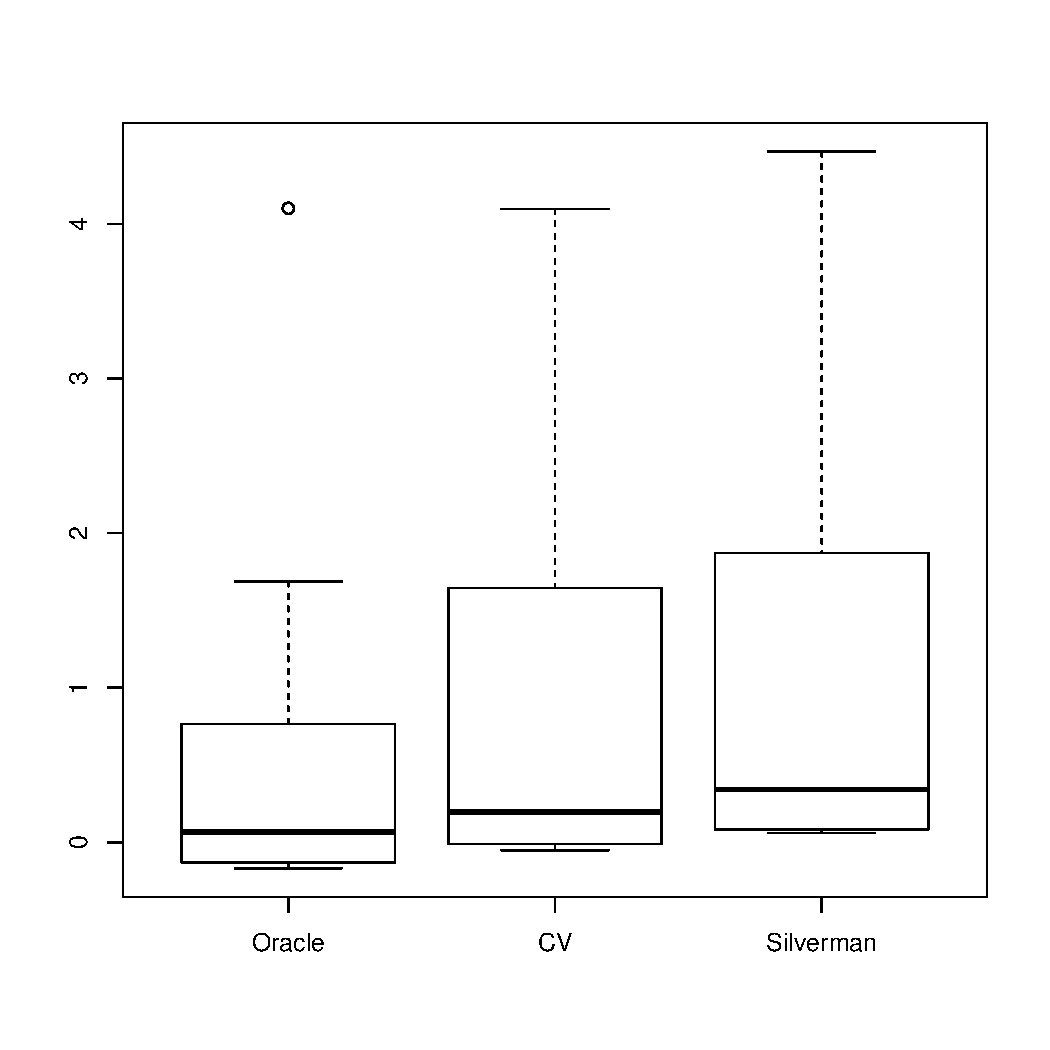
\includegraphics[width=\textwidth]{results/by_overall/relative-peak-bias-peakpop-boxplot}
        \subcaption{Peaked populations}
        \label{fig:discussion:overall_peakbias_boxplot:peak}
    \end{subfigure}
    \caption{Overall distribution of relative \glsentryname{peak bias}}
    \label{fig:discussion:overall_peakbias_boxplot}
\end{figure}

\begin{figure}[htbp]
    \centering
    \begin{subfigure}[t]{0.45\textwidth}
        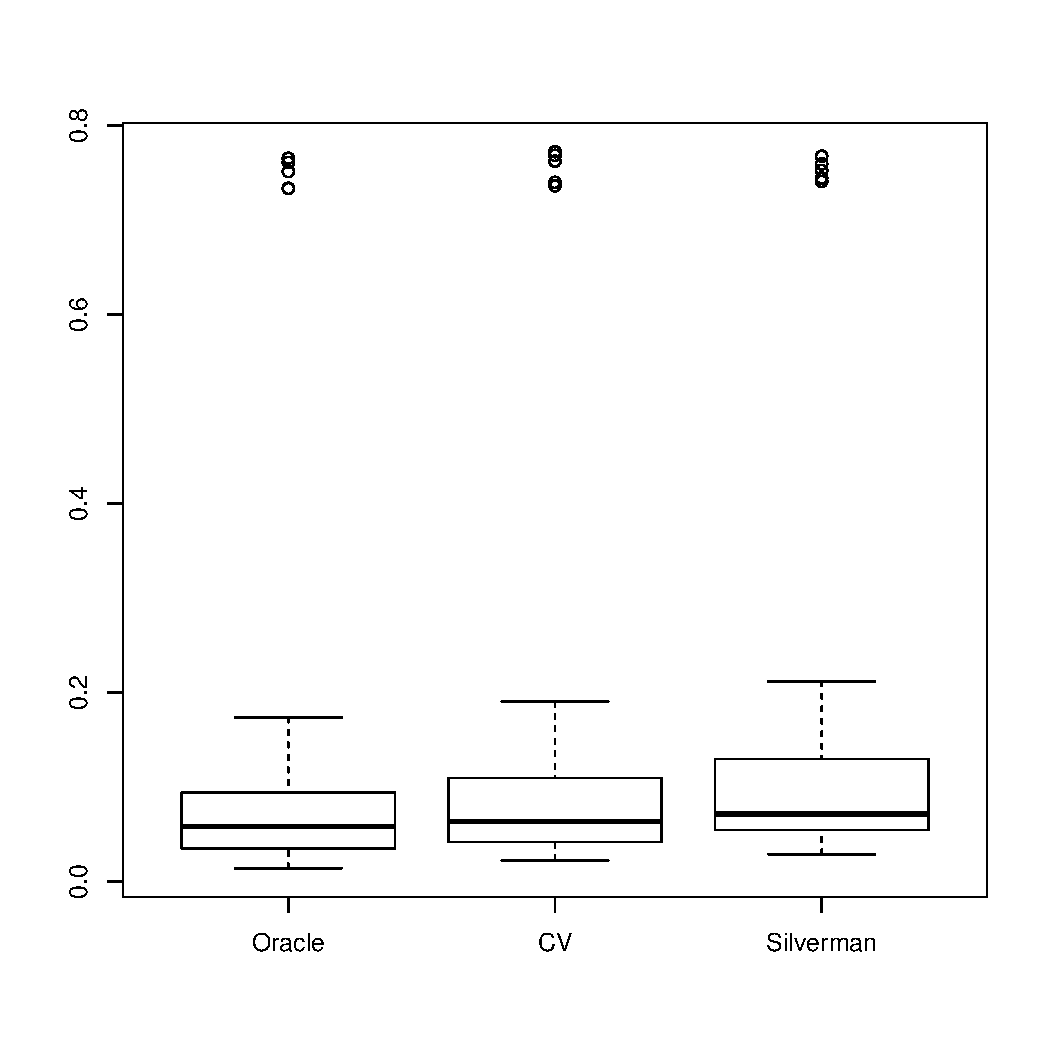
\includegraphics[width=\textwidth]{results/by_overall/relative-peak-drift-boxplot}
        \subcaption{Uniform populations}
        \label{fig:discussion:overall_peakdrift_boxplot:unif}
    \end{subfigure}
    \begin{subfigure}[t]{0.45\textwidth}
        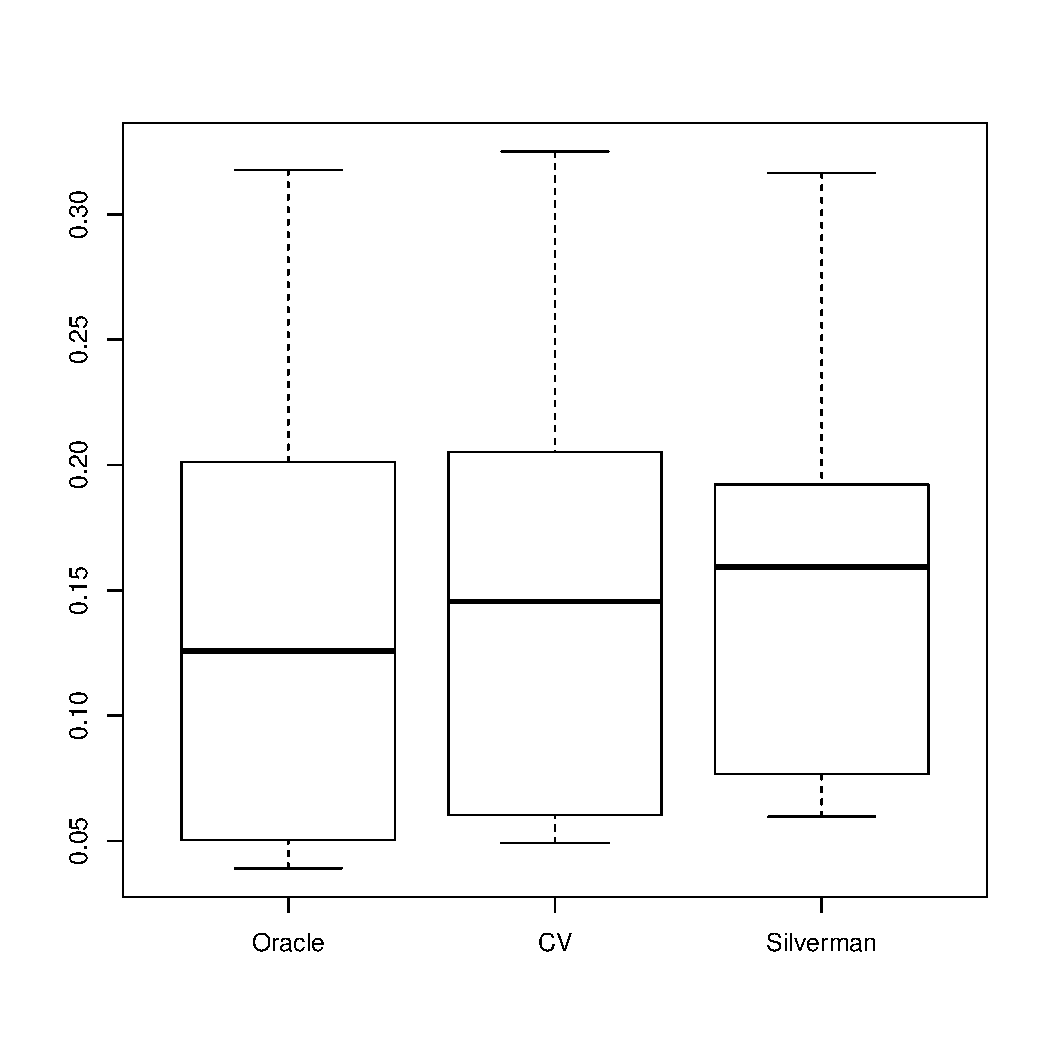
\includegraphics[width=\textwidth]{results/by_overall/relative-peak-drift-peakpop-boxplot}
        \subcaption{Peaked populations}
        \label{fig:discussion:overall_peakdrift_boxplot:peak}
    \end{subfigure}
    \caption{Overall distribution of relative \glsentryname{peak drift}}
    \label{fig:discussion:overall_peakdrift_boxplot}
\end{figure}

The distributions we observed for \gls{peak bias} and \gls{peak drift} are in \Cref{fig:discussion:overall_peakbias_boxplot,fig:discussion:overall_peakdrift_boxplot}.
First, we note that the \gls{peak bias} nearly always takes negative values when computing the \gls{dkd} with the \gls{oracle} bandwidth,
for uniformly distributed populations.


\begin{figure}[htbp]
    \centering
    \begin{subfigure}[t]{0.45\textwidth}
        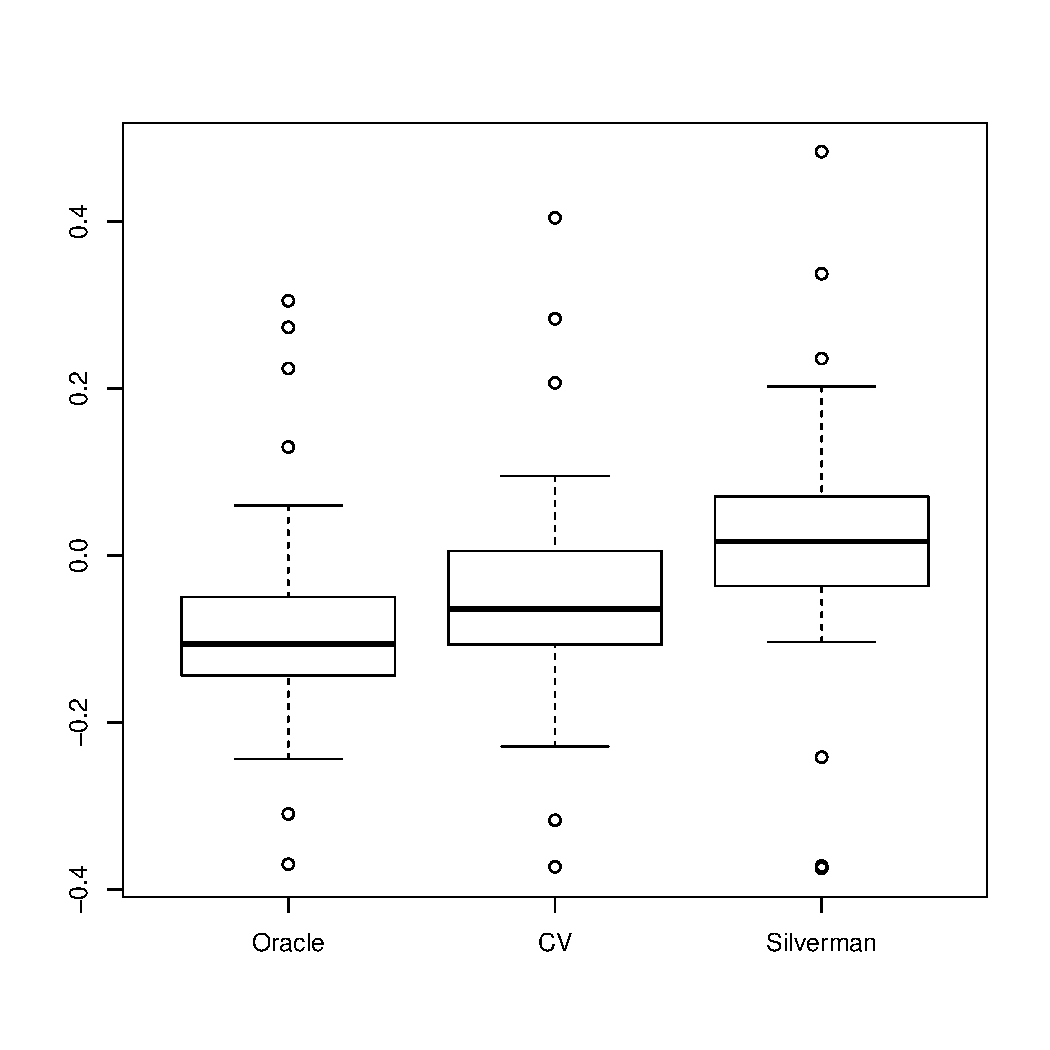
\includegraphics[width=\textwidth]{results/by_overall/relative-centroid-bias-boxplot}
        \subcaption{Uniform populations}
        \label{fig:discussion:overall_centroidbias_boxplot:unif}
    \end{subfigure}
    \begin{subfigure}[t]{0.45\textwidth}
        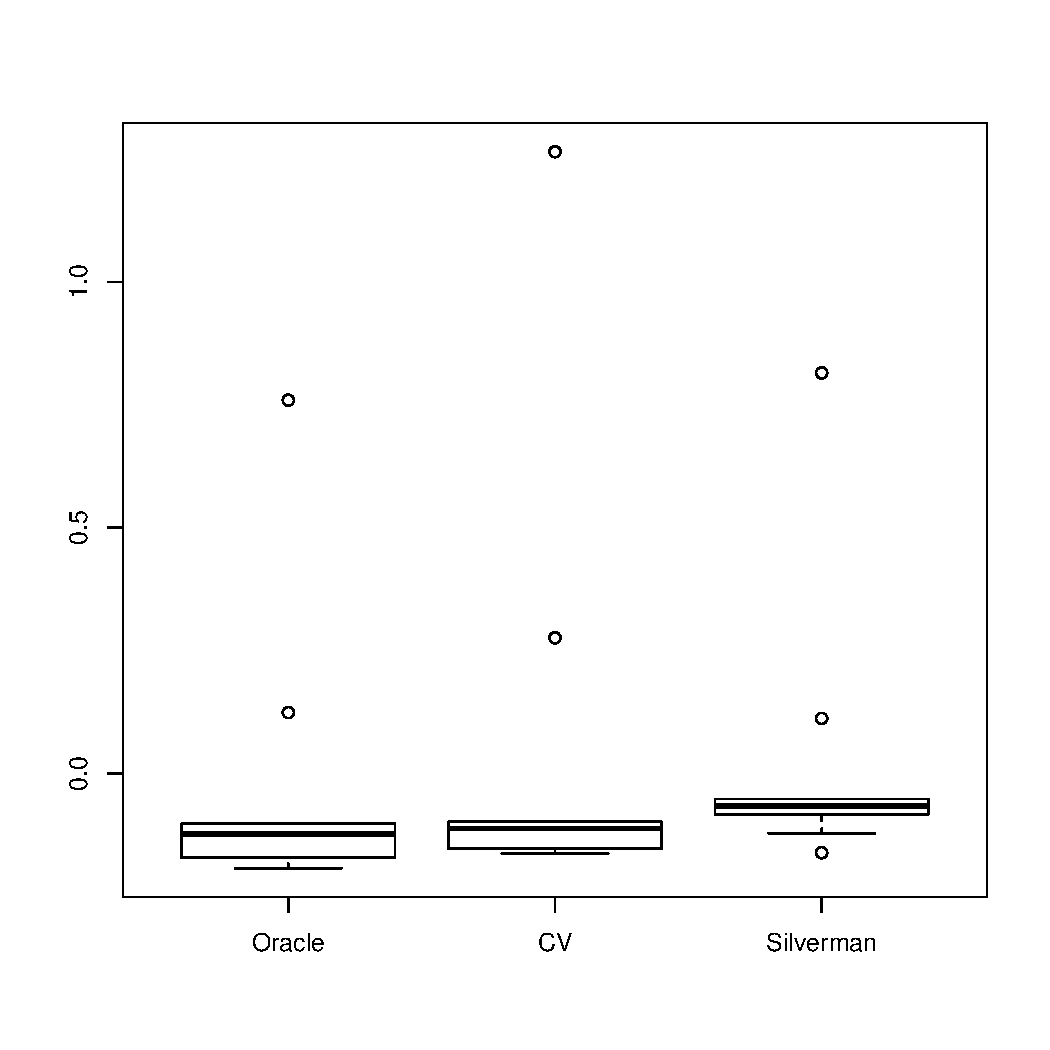
\includegraphics[width=\textwidth]{results/by_overall/relative-centroid-bias-peakpop-boxplot}
        \subcaption{Peaked populations}
        \label{fig:discussion:overall_centroidbias_boxplot:peak}
    \end{subfigure}
    \caption{Overall distribution of relative \glsentryname{centroid bias}}
    \label{fig:discussion:overall_centroidbias_boxplot}
\end{figure}

\begin{figure}[htbp]
    \centering
    \begin{subfigure}[t]{0.45\textwidth}
        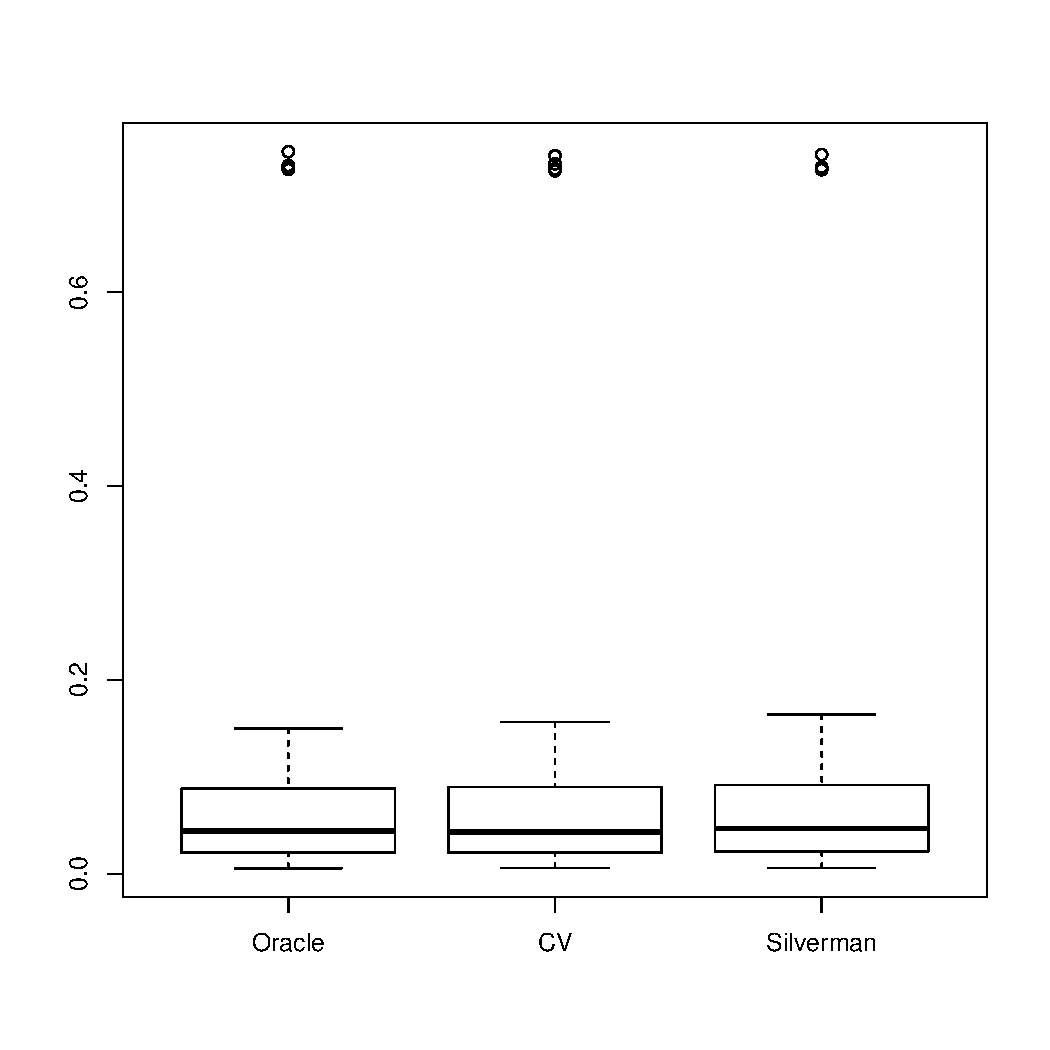
\includegraphics[width=\textwidth]{results/by_overall/relative-centroid-drift-boxplot}
        \subcaption{Uniform populations}
        \label{fig:discussion:overall_centroiddrift_boxplot:unif}
    \end{subfigure}
    \begin{subfigure}[t]{0.45\textwidth}
        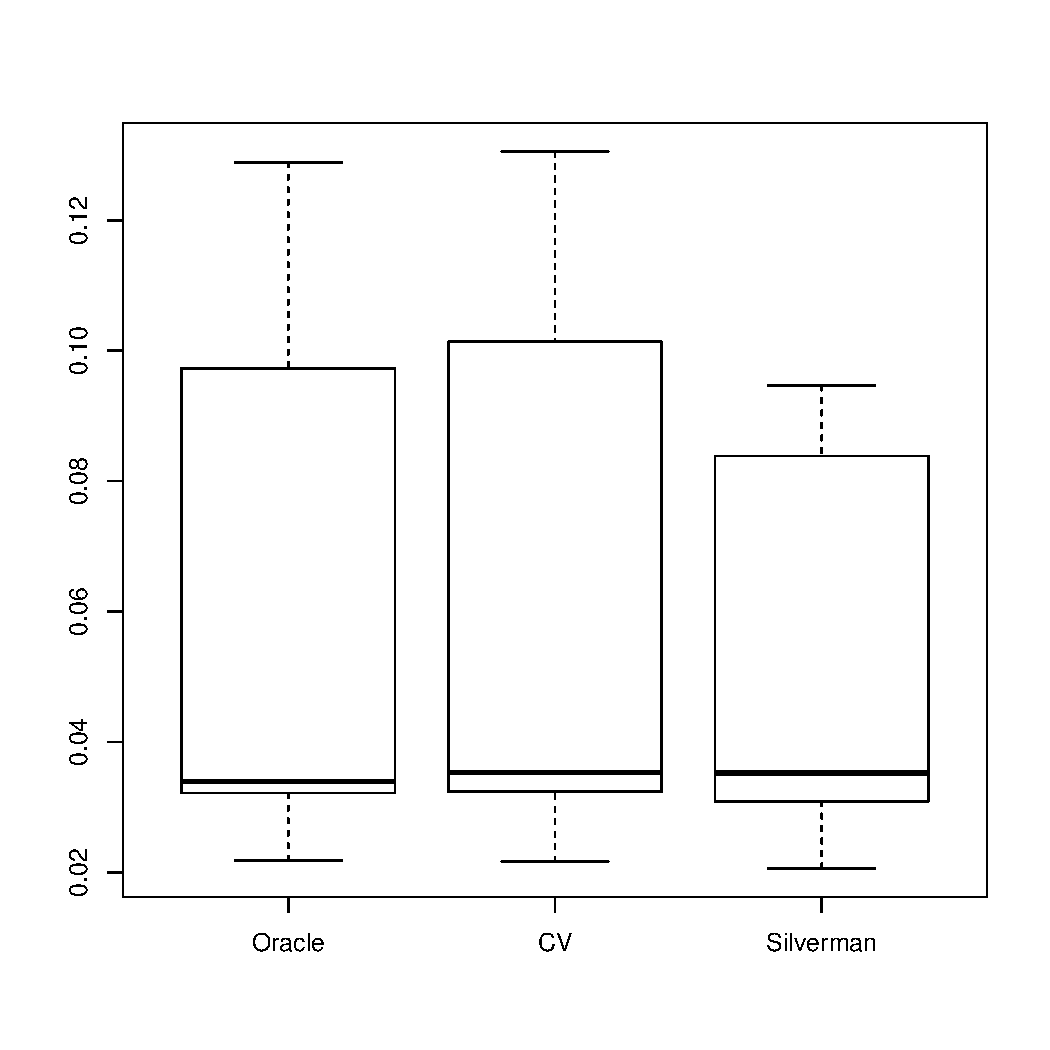
\includegraphics[width=\textwidth]{results/by_overall/relative-centroid-drift-peakpop-boxplot}
        \subcaption{Peaked populations}
        \label{fig:discussion:overall_centroiddrift_boxplot:peak}
    \end{subfigure}
    \caption{Overall distribution of relative \glsentryname{centroid drift}}
    \label{fig:discussion:overall_centroiddrift_boxplot}
\end{figure}

\section{Gradient descent for cross-validation}
\label{sec:discussion:gradient_descent}

We attempted to speed up the cross-validation bandwidth selection by using gradient descent.
We found the gradient descent algorithm often resulted in severe oversmoothing,
as the cross-validation error would decrease slowly as the bandwidth increased.
This required a lot of manual tuning of the learning rate parameter, and so required re-running the experiment several times.
We added \textit{momentum} to our gradient descent implementation but it did not help in every case, and so we changed our strategy to the one described in \Cref{ch:method}.

\section{Accuracy using Silverman}

In \Cref{tab:mean_error_rates:p0.7_100_1.0_1h} we see that the accuracy measure \gls{mise} using the \gls{silverman} rule of thumb is even better than was obtained using the \gls{oracle}.
We tried to run with an additional experiment with 499 monte carlo simulations, and found that in this case the \gls{silverman} rule did not outperform the \gls{oracle}.

